%===========================================================
\chapter{Climate Rescue: Can Evolution Outrun Warming?}
\label{ch:climate}
%===========================================================

\note{Climate forcing is observed data; the organism is a generic model, not a
calibrated real species.}

\section{The question and its theory}
\emph{Evolutionary rescue} is the recovery of a declining population through
adaptive genetic change (Gomulkiewicz \& Holt 1995; Bell \& Gonzalez 2009).
Quantitative-genetic theory (Lynch \& Lande 1993; B\"urger \& Lynch 1995) predicts
a critical rate of environmental change: below it the mean phenotype settles at a
constant lag behind a moving optimum; above it the lag grows until extinction. The
climate module measures that rate in Vikasa's individual-based world, then adds a
real-data climate twin, a Sobol sensitivity analysis, a Gaussian-process surrogate
and an offline HTML report with a SHA-256 manifest. The model is described here
following the ODD protocol (Grimm et al.\ 2006, 2020).

\section{ODD description}
\subsection{Purpose and patterns}
Estimate the warming rate in $^{\circ}$C per generation beyond which a population
with heritable thermal tolerance can no longer persist, and how much of persistence
is due to evolution. Expected patterns: survival falls as the rate rises;
heritability raises the tolerable rate; the evolved shift tracks warming at slow
rates; the adaptation lag grows with the rate.

\subsection{Entities, state variables and scales}
Animals carry the six body genes, temperament, energy, injury and age, plus a
thermal optimum $\theta$ ($^{\circ}$C) and current stress $\varsigma\in[0,1)$. The
environment carries $T(t)$ in $^{\circ}$C. Space is a $480\times320$ 2D world with
tens of animals; time is in ticks, and results are reported per measured generation.

\subsection{Process overview}
The ordinary Vikasa tick (Algorithm~\ref{alg:tick-doc}) runs unchanged. Thermal
stress is computed in the energy step, before the basal cost, and affects
reproduction eligibility and the cause assigned to injury deaths in the same tick.

\subsection{Design concepts}
Thermal performance is an asymmetric Gaussian (Huey \& Kingsolver 1989). With
$\Delta T=T-\theta$:
\[
\varsigma=1-\exp\!\left(-\frac{\Delta T^2}{2w^2}\right),\qquad
w=\begin{cases}0.6\,\omega&\Delta T>0\ \text{(warm side)}\\ \omega&\Delta T\le0\end{cases}
\]
The costs of stress are: basal cost $\times(1+1.5\varsigma)$; injury
$+0.02(\varsigma-0.3)/0.7$ per tick when $\varsigma>0.3$; and no breeding while
$\varsigma>0.7$ (heat-induced sterility; Walsh et al.\ 2019). Inheritance follows
the infinitesimal model (Section 6.4); the control arm has zero heritability.

\begin{figure}[htbp]
\centering
\begin{tikzpicture}
\draw[->] (-4.2,0) -- (4.4,0) node[right]{\small $\Delta T=T-\theta$ ($^{\circ}$C)};
\draw[->] (0,0) -- (0,3.4) node[above]{\small stress $\varsigma$};
\foreach \x in {-4,-2,2,4} \draw (\x,0.06)--(\x,-0.06) node[below]{\scriptsize \pgfmathparse{int(\x*2)}\pgfmathresult};
\draw[thick,vk,domain=-4:0,samples=80] plot (\x,{3*(1-exp(-(2*\x)^2/(2*16)))});
\draw[thick,red!70!black,domain=0:4,samples=80] plot (\x,{3*(1-exp(-(2*\x)^2/(2*(0.6*4)^2)))});
\draw[dashed,gray] (-4.2,2.1) -- (4.2,2.1) node[right,font=\scriptsize]{0.7 breeding stops};
\draw[dashed,gray!60] (-4.2,0.9) -- (4.2,0.9) node[right,font=\scriptsize]{0.3 injury starts};
\node[font=\scriptsize,vk] at (-2.6,2.7) {cold side $w=\omega$};
\node[font=\scriptsize,red!70!black] at (2.4,3.2) {warm side $w=0.6\omega$};
\end{tikzpicture}
\caption{Asymmetric thermal stress for $\omega=4\,^{\circ}$C. The warm side
reaches the breeding limit at $\Delta T\approx+3.7\,^{\circ}$C, the cold side only
at $\approx-6.2\,^{\circ}$C.}
\end{figure}

\subsection{Initialisation and input data}
Founders draw $\theta\sim\mathcal{N}(\bar T+\Delta_0,1\,^{\circ}\mathrm{C})$. World,
resources and population come from \code{config/climate-rescue.json}. Temperature is
\[
T(t)=T_{\text{clim}}\big(\text{month}(t)\big)+\Delta\big(\text{year}(t)\big),
\]
where $T_{\text{clim}}$ is the 1991--2020 monthly climatology of NASA POWER 2\,m
air temperature (MERRA-2 reanalysis), retrieved for 1981--2025. Each region file
stores the raw series, climatology, an OLS trend $\pm$ SE and provenance (URL,
retrieval time, SHA-256 of the response); a climatology needs at least 20 years.
The anomaly $\Delta$ is linear from 2005 (the centre of 1995--2014) to 2090 (the
centre of 2081--2100) and reaches the IPCC AR6 WG1 Chapter~4 Table~4.5 medians,
optionally multiplied by a regional factor.

\begin{table}[htbp]
\centering
\caption{IPCC AR6 warming medians and derived rates}
\begin{tabular}{lcc}
\toprule
Pathway & 2081--2100 vs 1995--2014 & Linear rate ($^{\circ}$C/yr) \\
\midrule
SSP1-2.6 & 0.9\,$^{\circ}$C & 0.011 \\
SSP2-4.5 & 1.8\,$^{\circ}$C & 0.021 \\
SSP3-7.0 & 2.8\,$^{\circ}$C & 0.033 \\
SSP5-8.5 & 3.5\,$^{\circ}$C & 0.041 \\
\bottomrule
\end{tabular}
\end{table}

\begin{table}[htbp]
\centering
\caption{Published study regions}
\begin{tabular}{lccc}
\toprule
Region & Annual mean & Seasonal amplitude & Trend 1981--2025 ($^{\circ}$C/decade) \\
\midrule
Western Ghats (Agumbe) & 25.3 & 2.4 & $+0.169\pm0.029$ \\
Delhi NCR & 25.6 & 11.1 & $-0.120\pm0.068$ \\
Sundarbans & 26.2 & 5.4 & $-0.002\pm0.030$ \\
\bottomrule
\end{tabular}
\end{table}
The slight Delhi cooling is reported as measured; it is consistent with aerosol
and haze dimming over the Indo-Gangetic plain in MERRA-2 and is not a forecast.

\subsection{Submodels and calibration}
The generation interval is $1/$slope of mean living ancestral depth per tick at
zero warming, averaged over three calibration seeds (901, 902, 903; 1{,}500
burn-in and 6{,}000 measured ticks): $G=469$ ticks. The rescue protocol has 5
generations of burn-in, 20 of warming at rate $r$ and 5 of hold, with one climate
year per generation, Western Ghats climatology and $\omega=4\,^{\circ}$C.
Outcomes: survival, extinction generation, population before warming, at minimum
and at the end, evolved shift in mean $\theta$, adaptation lag over the last five
warming generations, and the rescue signature (dip below 50\% then recovery to
$\ge80\%$). For the sweep the monthly cycle is a sinusoid whose half-range equals
the amplitude exactly.

\section{The pipeline}
\begin{lstlisting}
vikasa climate pipeline --profile full --root exports\climate\full
vikasa climate pipeline --profile quick --root exports\climate\quick
vikasa climate fetch --lat 18.52 --lon 73.86 --name Pune --key pune --output data\pune.json
vikasa climate assess --root exports\climate\full --region data\pune.json \
    --generation-years 2 --breadth 3 --ssp SSP2-4.5 --ssp SSP5-8.5
vikasa climate report --root exports\climate\full
\end{lstlisting}
The pipeline runs five resumable stages (calibrate, sweep, sensitivity, assess,
report) in parallel worker processes, appending results to JSON-lines files so an
interrupted run continues where it stopped. A root calibrated for one profile
refuses another.

\begin{table}[htbp]
\centering
\caption{Pipeline profiles}
\begin{tabularx}{\textwidth}{lLL}
\toprule
Setting & quick & full \\
\midrule
Rates ($^{\circ}$C/gen) & 0, 0.3, 1.2 & 0, 0.025, 0.05, 0.075, 0.1, 0.15, 0.2, 0.3, 0.4 \\
Seeds per cell & 3 & 12 \\
Phases (gens) & 2 / 4 / 2 & 5 / 20 / 5 \\
Calibration & 1 seed, 500 + 1{,}500 ticks & 3 seeds, 1{,}500 + 6{,}000 ticks \\
Design / hold-out points & 24 / 8 & $2\times192$ / 48 \\
Sobol $n$, bootstrap & 1{,}024, 200 & 4{,}096, 2{,}000 \\
Regions, SSPs & Western Ghats; 2 SSPs & 3 regions; 4 SSPs \\
Assessment seeds, cap & 3, 4 gens & 12, 40 gens; local breadth $1.5\times$ \\
\bottomrule
\end{tabularx}
\end{table}

\section{Statistics}
\begin{itemize}[leftmargin=*]
\item \textbf{Critical rate.} A lightly penalised logistic regression (L2, $C=10$
on the rate scaled by its maximum, L-BFGS) fits $\mathrm{logit}\,p=\beta_0+\beta_1r$,
finite even under perfect separation. $k_c=-\beta_0/\beta_1$ is accepted only if
$\beta_1<0$ and $0\le k_c\le2r_{\max}$. A 2{,}000-resample bootstrap gives the CI.
\item \textbf{Rescue gain.} Paired bootstrap over seeds of $k_c^{\text{her}}-k_c^{\text{ctl}}$.
\item \textbf{Lag regression.} Pearson correlation and slope of lag against rate over surviving heritable runs.
\item \textbf{Sensitivity.} Six inputs (Table~\ref{tab:sobolparams}) sampled by Latin
hypercube. A GP regressor with kernel $\text{Const}\times\text{Mat\'ern}_{5/2}(\ell=0.3)+\text{White}(0.01)$
models the final/pre-warming population ratio, clipped to $[0,2]$. Survival
probability is $P(\text{ratio}>\tau)$ under the predictive normal, where $\tau$ is
the midpoint between the largest extinct and smallest surviving training ratio.
Five-fold CV and hold-out $R^2$, AUC and Brier score assess it.
\item \textbf{Sobol indices.} Scrambled Sobol (Saltelli) base samples $A,B$ with
$n=4{,}096$, $AB_i$ swapping column $i$, Jansen estimators
$S_i=(V-\tfrac12\mathbb{E}[(f_B-f_{AB_i})^2])/V$ and
$S_{T,i}=\tfrac12\mathbb{E}[(f_A-f_{AB_i})^2]/V$, 200 bootstrap resamples; the
estimator is unit-tested on the Ishigami function.
\end{itemize}

\begin{table}[htbp]
\centering
\caption{Sensitivity inputs}
\label{tab:sobolparams}
\begin{tabular}{llc}
\toprule
Input & Meaning & Range \\
\midrule
\code{rate\_c\_per\_gen} & Warming rate & 0 -- $r_{\text{high}}$ \\
\code{breadth\_c} & Cold-side tolerance breadth & 2 -- 8\,$^{\circ}$C \\
\code{amplitude\_c} & Seasonal amplitude & 0.5 -- 8\,$^{\circ}$C \\
\code{founder\_sd\_c} & Standing variation in $\theta$ & 0.25 -- 2\,$^{\circ}$C \\
\code{segregation\_sd\_c} & Heritable offspring variation & 0 -- 1\,$^{\circ}$C \\
\code{capacity\_scale} & Carrying-capacity multiplier & 0.5 -- 1.5 \\
\bottomrule
\end{tabular}
\end{table}

\section{Results}
All numbers come from \code{docs/results/climate-rescue-2026-10-18/}.

\begin{table}[htbp]
\centering
\caption{Critical warming rate}
\begin{tabular}{lcc}
\toprule
Arm & $k_c$ ($^{\circ}$C/generation) & 95\% CI \\
\midrule
Heritable thermal tolerance & \textbf{0.262} & 0.234--0.291 \\
Control: same variation, no heritability & 0.067 & 0.052--0.080 \\
Rescue gain (paired bootstrap) & \textbf{+0.196} & 0.165--0.230 \\
\bottomrule
\end{tabular}
\end{table}

\begin{figure}[htbp]
\centering
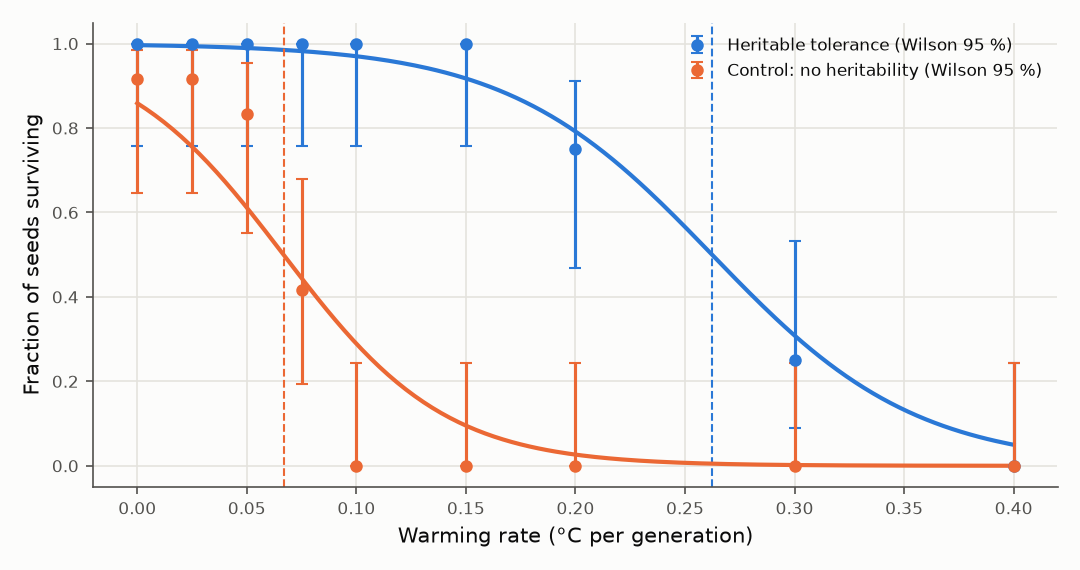
\includegraphics[width=0.82\textwidth]{survival_curve.png}
\caption{Survival against warming rate, heritable vs control, with Wilson intervals and logistic fits.}
\end{figure}

Heritable populations survived every seed up to 0.15, 9/12 at 0.2, 3/12 at 0.3
and none at 0.4\,$^{\circ}$C/gen; controls began failing at 0.075 and none
survived 0.1. The evolved shift was $+1.2$, $+2.9$ and $+4.5\,^{\circ}$C at 0.1,
0.2 and 0.3 (against 2, 4 and 6\,$^{\circ}$C of warming). Lag rose linearly with
slope 6.4\,$^{\circ}$C per ($^{\circ}$C/gen), $r=0.85$, $n=81$. Near $k_c$,
17--25\% of surviving runs showed the rescue signature.

\begin{figure}[htbp]
\centering
\begin{minipage}{0.49\textwidth}\centering
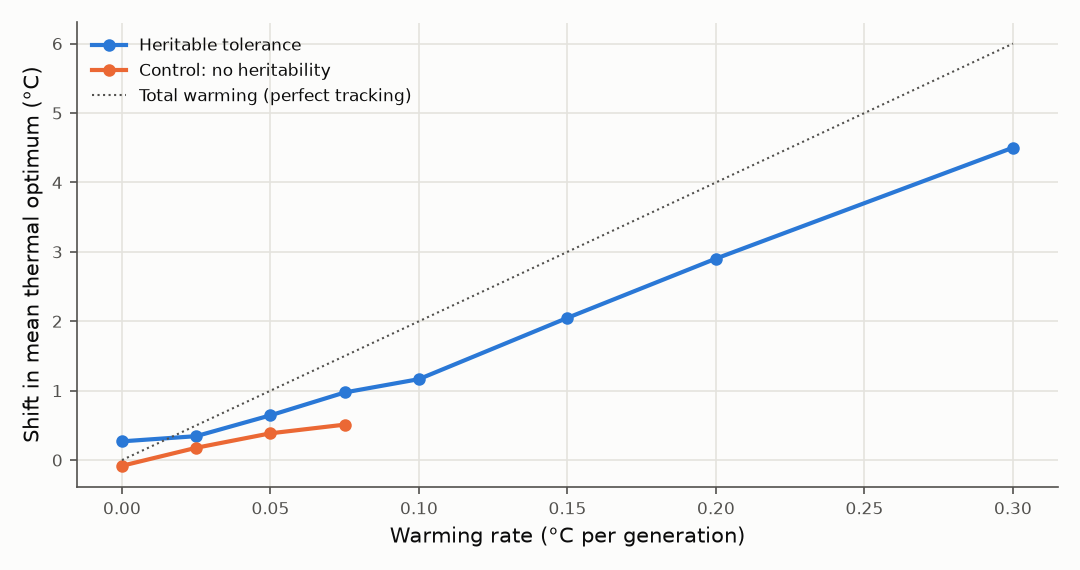
\includegraphics[width=\linewidth]{shift_vs_rate.png}\\[-2pt]
{\small (a) Evolved shift in mean optimum}
\end{minipage}\hfill
\begin{minipage}{0.49\textwidth}\centering
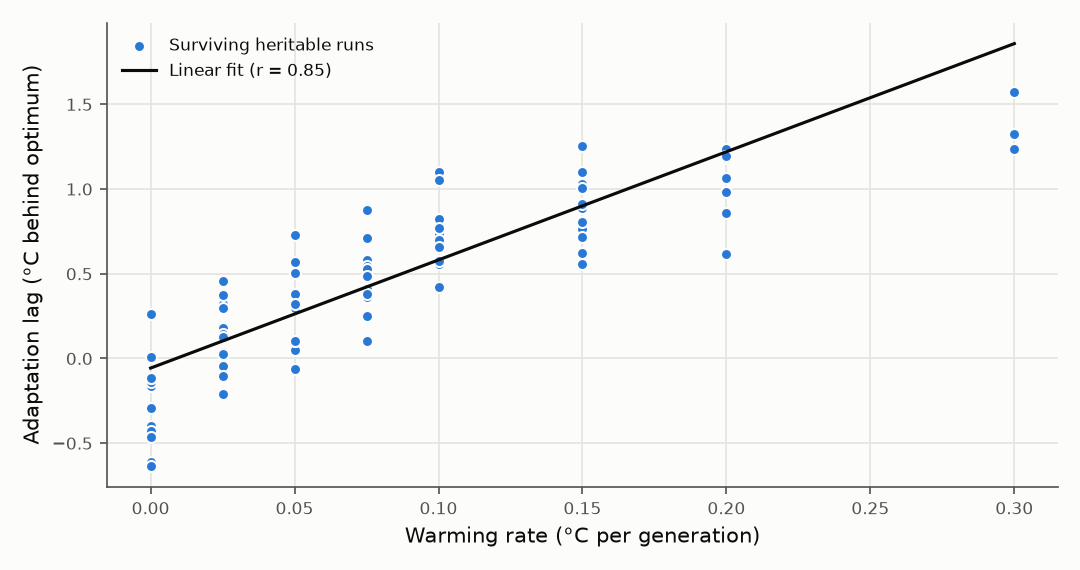
\includegraphics[width=\linewidth]{lag_vs_rate.png}\\[-2pt]
{\small (b) Adaptation lag}
\end{minipage}
\caption{Shift and lag versus warming rate.}
\end{figure}

\begin{figure}[htbp]
\centering
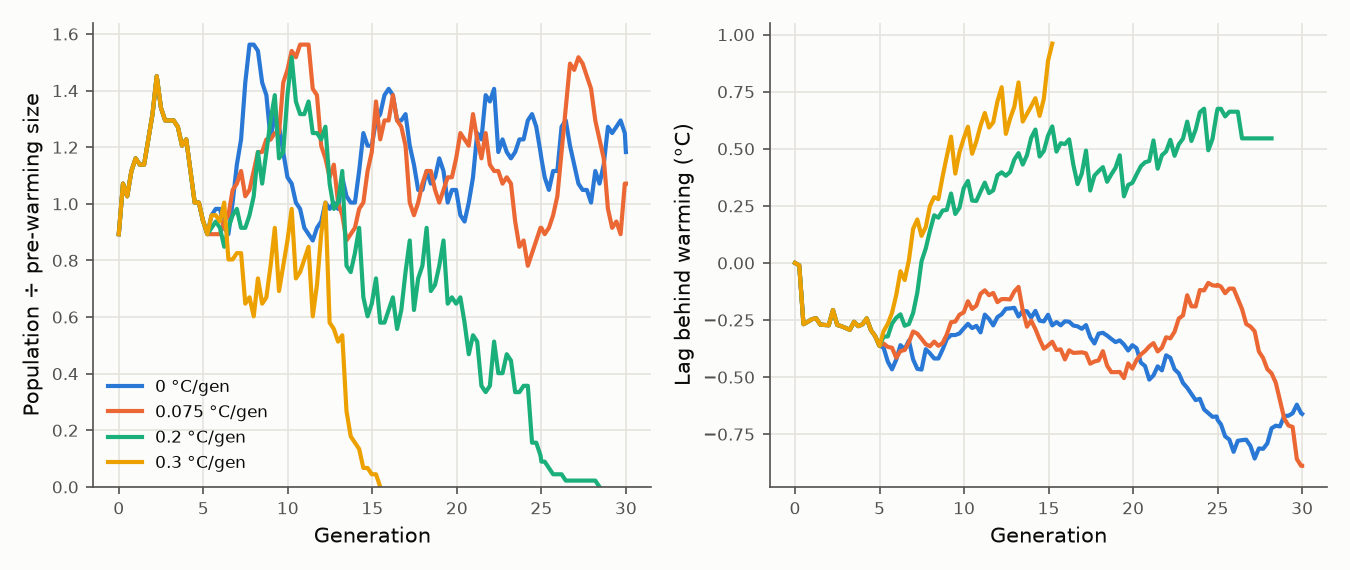
\includegraphics[width=0.95\textwidth]{trajectories.png}
\caption{Population and lag trajectories through burn-in, warming and hold.}
\end{figure}

\begin{figure}[htbp]
\centering
\begin{minipage}{0.56\textwidth}\centering
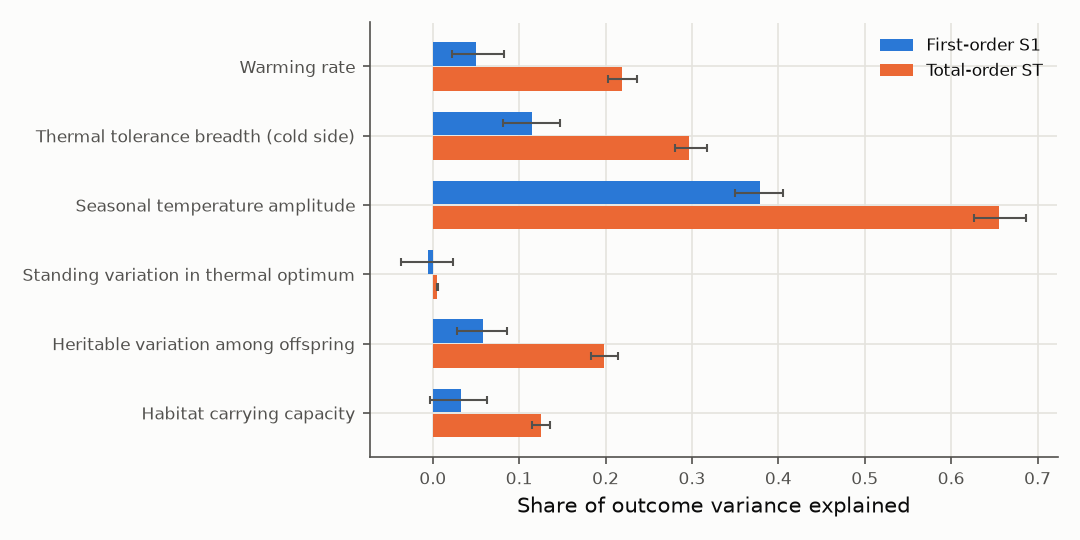
\includegraphics[width=\linewidth]{sobol_bars.png}\\[-2pt]
{\small (a) Sobol indices}
\end{minipage}\hfill
\begin{minipage}{0.4\textwidth}\centering
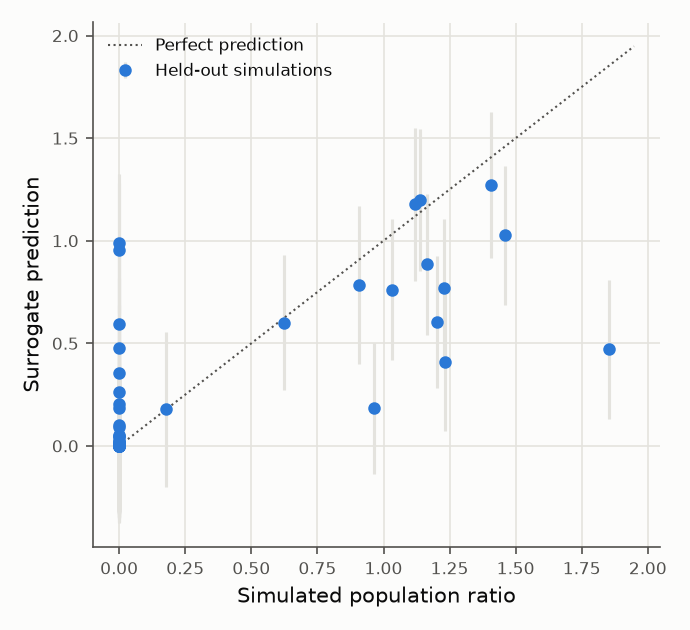
\includegraphics[width=\linewidth]{surrogate_parity.png}\\[-2pt]
{\small (b) Surrogate parity}
\end{minipage}
\caption{Sensitivity: total-order indices were amplitude 0.66, breadth 0.30, rate
0.22, segregation SD 0.20, capacity 0.13, standing variation $\approx0$.}
\end{figure}

\begin{table}[htbp]
\centering
\caption{Regional viability}
\begin{tabularx}{\textwidth}{lLL}
\toprule
Region & Reference organism ($\omega=4$) & Locally adapted ($1.5\times$ amplitude) \\
\midrule
Western Ghats & persists under all SSPs ($p=0.92$--$1.0$) & same as reference \\
Delhi NCR & not viable even without warming & $\omega=16.6$: persists, $p=0.92$--$1.0$ \\
Sundarbans & not viable even without warming & $\omega=8.2$: persists, $p=1.0$ \\
\bottomrule
\end{tabularx}
\end{table}

\begin{table}[htbp]
\centering
\caption{Critical generation time $=k_c\,/\,$warming per year}
\begin{tabular}{lcc}
\toprule
Scenario & Warming ($^{\circ}$C/yr) & Critical generation time (yr, 95\% CI) \\
\midrule
SSP1-2.6 & 0.011 & 24.8 (22.1--27.5) \\
SSP2-4.5 & 0.021 & 12.4 (11.0--13.7) \\
SSP3-7.0 & 0.033 & 8.0 (7.1--8.8) \\
SSP5-8.5 & 0.041 & 6.4 (5.7--7.1) \\
\bottomrule
\end{tabular}
\end{table}

Checked by direct simulation (Western Ghats, real monthly cycle, 2025--2100, 12
seeds): six-year species survive with $p=1.00$ (SSP2-4.5), 0.67 (SSP3-7.0) and
0.50 (SSP5-8.5, where 0.247\,$^{\circ}$C/gen $\approx k_c$); twelve-year species
0.92, 0.50 and 0.25. Twelve-year species beat the simple rule because 2025--2100
spans only about six generations, so the critical generation time is conservative
for long-lived species over this century.

\begin{figure}[htbp]
\centering
\begin{minipage}{0.49\textwidth}\centering
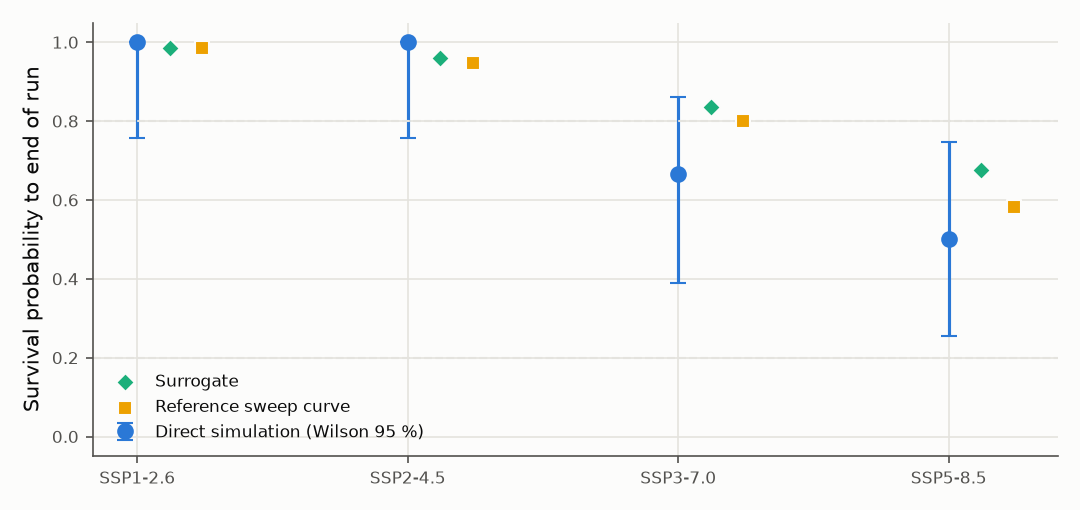
\includegraphics[width=\linewidth]{assessment_western-ghats-g6.png}\\[-2pt]
{\small (a) Six-year generations}
\end{minipage}\hfill
\begin{minipage}{0.49\textwidth}\centering
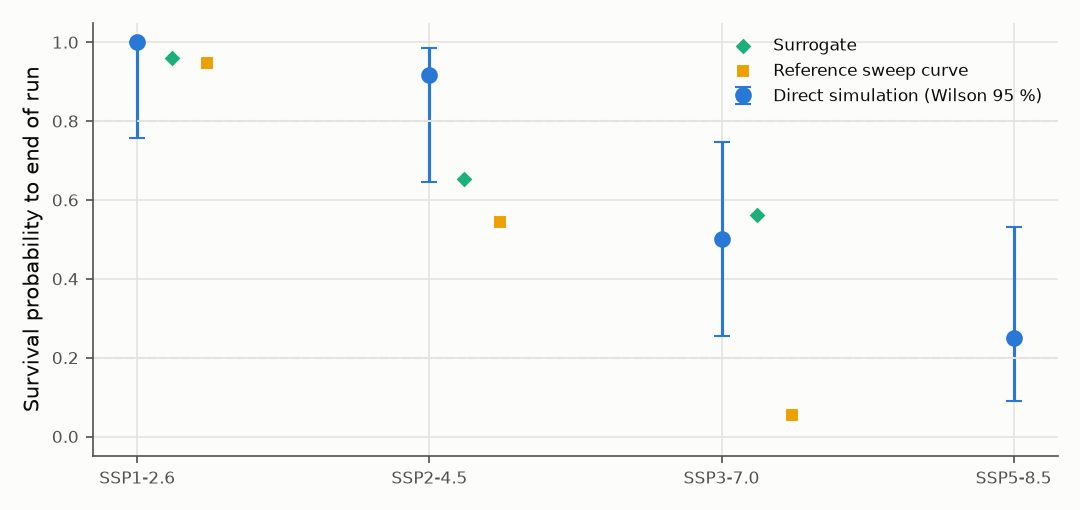
\includegraphics[width=\linewidth]{assessment_western-ghats-g12.png}\\[-2pt]
{\small (b) Twelve-year generations}
\end{minipage}
\caption{Direct regional assessments, Western Ghats.}
\end{figure}

\section{Pre-registered success criteria}
\begin{longtable}{p{0.8cm}p{1.2cm}p{12.4cm}}
\caption{Criteria fixed before the production run}\\
\toprule
ID & Result & Criterion and outcome \\
\midrule
\endfirsthead
C1 & PASS & Populations persist without warming: 12/12. \\
C2 & PASS & Faster warming lowers survival: Spearman $\rho=-0.84$. \\
C3 & PASS & Heritability raises $k_c$: gain CI 0.165--0.230. \\
C4 & FAIL & Optima track $\ge50\%$ of warming and $\ge2\times$ the control shift at $\le k_c/2$. The first holds, but controls also shift by about half as much: heat kills cold-adapted individuals within each generation, so the surviving control population's mean optimum moves although nothing is inherited. \\
C5 & PASS & Lag grows with rate: $r=0.85$. \\
C6 & PASS & No invariant violations or failed runs: 0/0. \\
S9 & FAIL & Surrogate hold-out $R^2\ge0.7$ and AUC $\ge0.85$: $R^2=0.51$, AUC $=0.93$ after the planned one-time escalation from 192 to 384 design runs. Even a perfect predictor explains at most about 78\% of single-run variance. \\
S10 & FAIL & Warming rate in the top two drivers: ranks third ($S_T=0.22$). \\
\bottomrule
\end{longtable}
No parameters were changed after the production run to make a criterion pass.

%===========================================================
\chapter{Species Risk Checker}
\label{ch:risk}
%===========================================================

\begin{figure}[htbp]
\centering
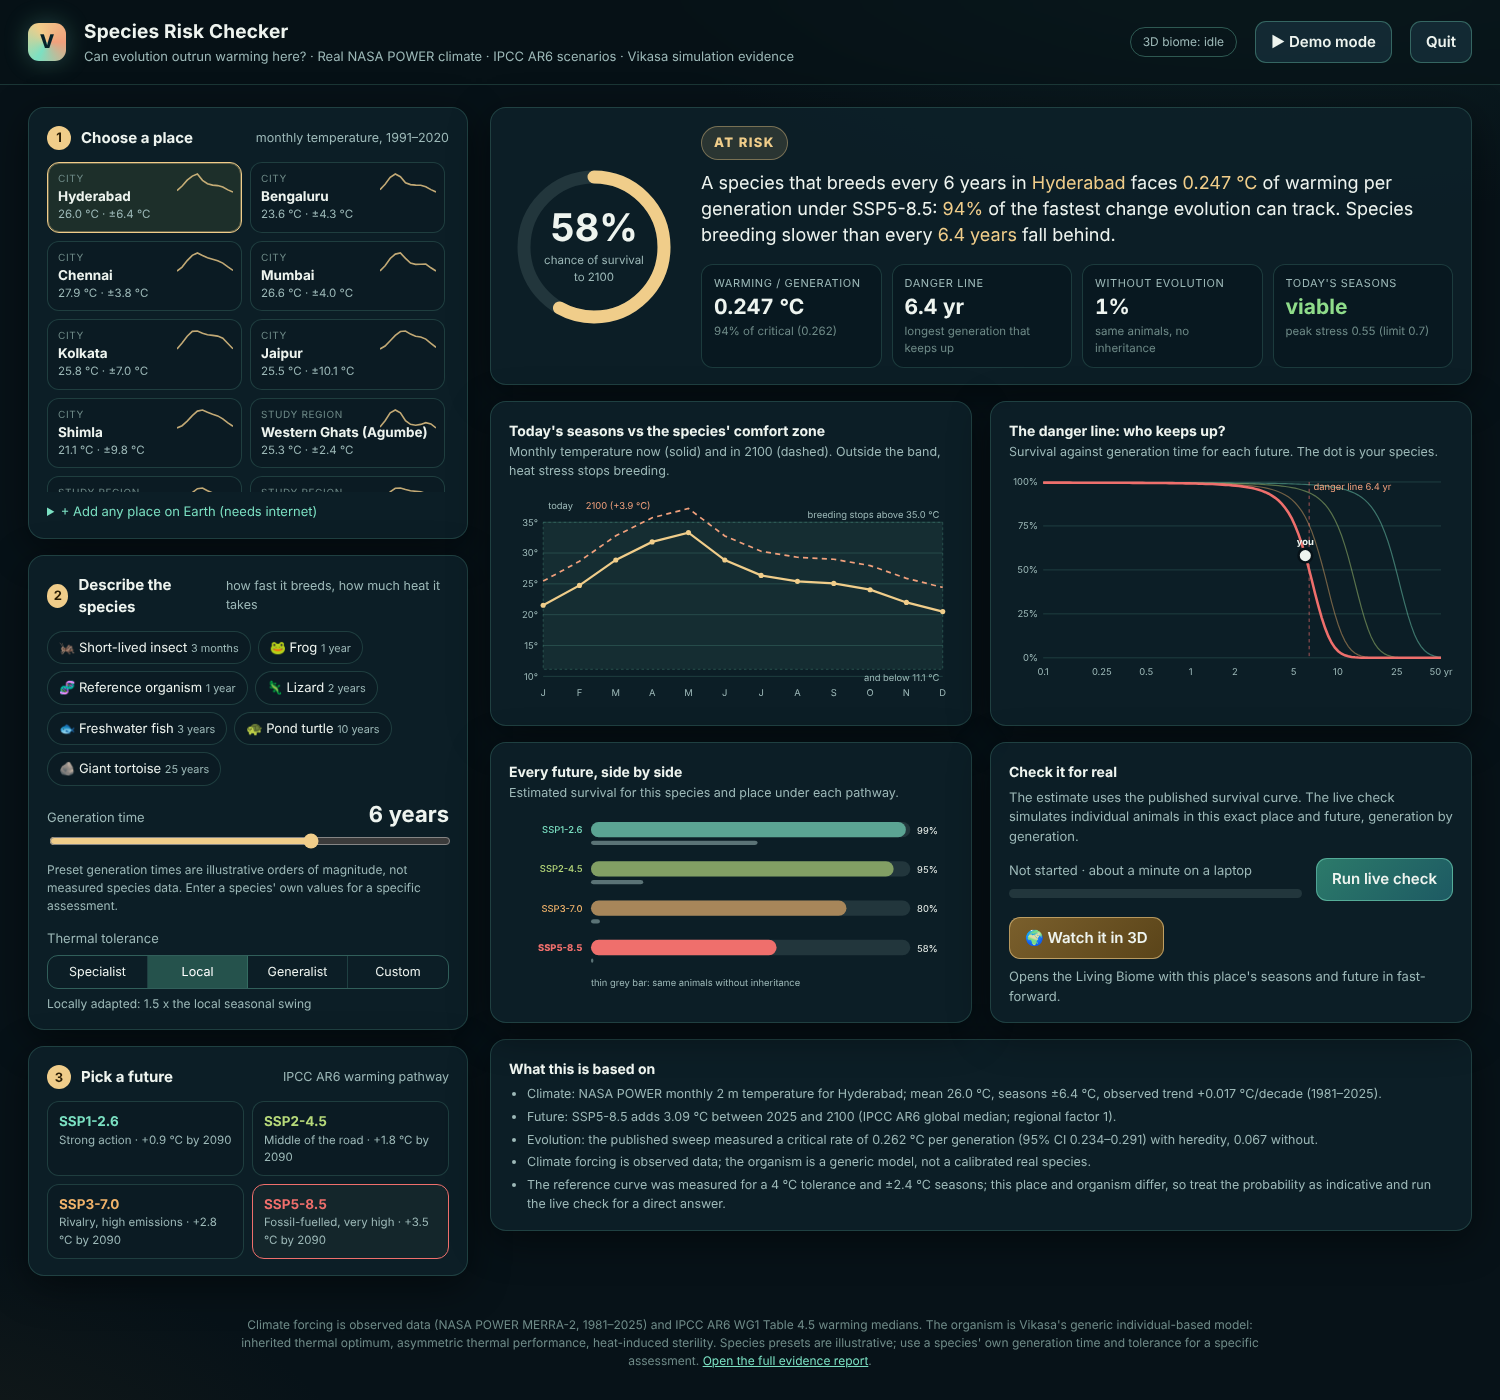
\includegraphics[width=0.5\textwidth]{risk-checker.png}
\caption{Species Risk Checker: a six-year species in Hyderabad under SSP5-8.5.}
\end{figure}

\section{Inputs}
\begin{table}[htbp]
\centering
\caption{Risk Checker inputs}
\begin{tabularx}{\textwidth}{lL}
\toprule
Input & Meaning and source \\
\midrule
Place & Monthly T2M climatology 1991--2020 and 1981--2025 trend from NASA POWER; bundled or fetched live for any latitude/longitude. \\
Generation time & Years from birth to the mean age of parents; presets from insect (3 months) to giant tortoise; range 0.05--50 years. \\
Tolerance & Breadth $\omega$: specialist $1\times$, local $1.5\times$ (default) or generalist $2.5\times$ the local seasonal swing, or a custom $^{\circ}$C value. \\
Future & SSP1-2.6, SSP2-4.5, SSP3-7.0 or SSP5-8.5. \\
\bottomrule
\end{tabularx}
\end{table}

\begin{table}[htbp]
\centering
\caption{Bundled Risk Checker places (reanalysis grid cells)}
\begin{tabular}{llccc}
\toprule
Key & Place & Mean ($^{\circ}$C) & Seasons ($\pm^{\circ}$C) & Trend ($^{\circ}$C/decade) \\
\midrule
\code{hyderabad} & Hyderabad & 26.0 & 6.4 & $+0.017$ \\
\code{bengaluru} & Bengaluru & 23.6 & 4.3 & $+0.092$ \\
\code{chennai} & Chennai & 27.9 & 3.8 & $+0.063$ \\
\code{mumbai} & Mumbai & 26.6 & 4.0 & $+0.127$ \\
\code{kolkata} & Kolkata & 25.8 & 7.0 & $-0.037$ \\
\code{jaipur} & Jaipur & 25.5 & 10.1 & $-0.075$ \\
\code{shimla} & Shimla & 21.1 & 9.8 & $-0.043$ \\
\code{western-ghats} & Western Ghats & 25.3 & 2.4 & $+0.169$ \\
\code{delhi-ncr} & Delhi NCR & 25.6 & 11.1 & $-0.120$ \\
\code{sundarbans} & Sundarbans & 26.2 & 5.4 & $-0.002$ \\
\bottomrule
\end{tabular}
\end{table}

\section{Instant estimate}
\textbf{Step 1, can it live here today?} Founders start at the annual mean; the
model's stress rule is applied to the hottest and coldest months:
\[
\varsigma_{\text{warm}}=1-e^{-(T_{\max}-\bar T)^2/2(0.6\omega)^2},\qquad
\varsigma_{\text{cold}}=1-e^{-(\bar T-T_{\min})^2/2\omega^2}.
\]
Peak stress above 0.75 is \emph{not viable}, 0.65--0.75 \emph{borderline} and below
0.65 \emph{viable}. With no fitted parameters this reproduces all five published
baseline verdicts (Western Ghats reference 0.53 viable; Sundarbans reference 0.78
not viable; Sundarbans local 0.30 viable; Delhi reference 1.00 not viable; Delhi
local 0.42 viable), enforced by
\code{test\_seasonal\_screen\_reproduces\_every\_published\_baseline\_verdict}.

\textbf{Step 2, can evolution keep up?} Warming per generation $=$ SSP rate per
year $\times$ generation time; survival with and without evolution comes from the
logistic curves stored with provenance in \code{climate/data/risk-reference.json}.
The danger line is $k_c$ divided by the warming per year.

\textbf{Domain check.} The curve was measured for $\omega=4\,^{\circ}$C and
$\pm2.4\,^{\circ}$C seasons. Inputs more than 25\% away are labelled
\emph{indicative}; rates above 0.4\,$^{\circ}$C/gen are \emph{extrapolated}.

\section{Live check and 3D replay}
\emph{Run live check} (\code{--live}) measures the generation interval in today's
climate (2 calibration seeds, 7{,}500 ticks), returns \emph{not viable in
present-day climate} if every calibration population dies, then runs 4 seeded
populations (5 burn-in, up to 25 warming, 5 hold generations) and reports survivors,
a Wilson interval and a verdict: $\ge80\%$ \emph{likely persists}, $\ge20\%$
\emph{at risk}, otherwise \emph{likely lost}. Results are cached under
\code{exports/risk/live/}. \emph{Watch it in 3D} writes a Living Biome world with
the place's real monthly cycle and the organism's breadth, applies warming each
climate year for 20 years after a 3-year settling period, and opens Godot with a
live temperature readout whose tooltip shows the adaptation lag.

\begin{figure}[htbp]
\centering
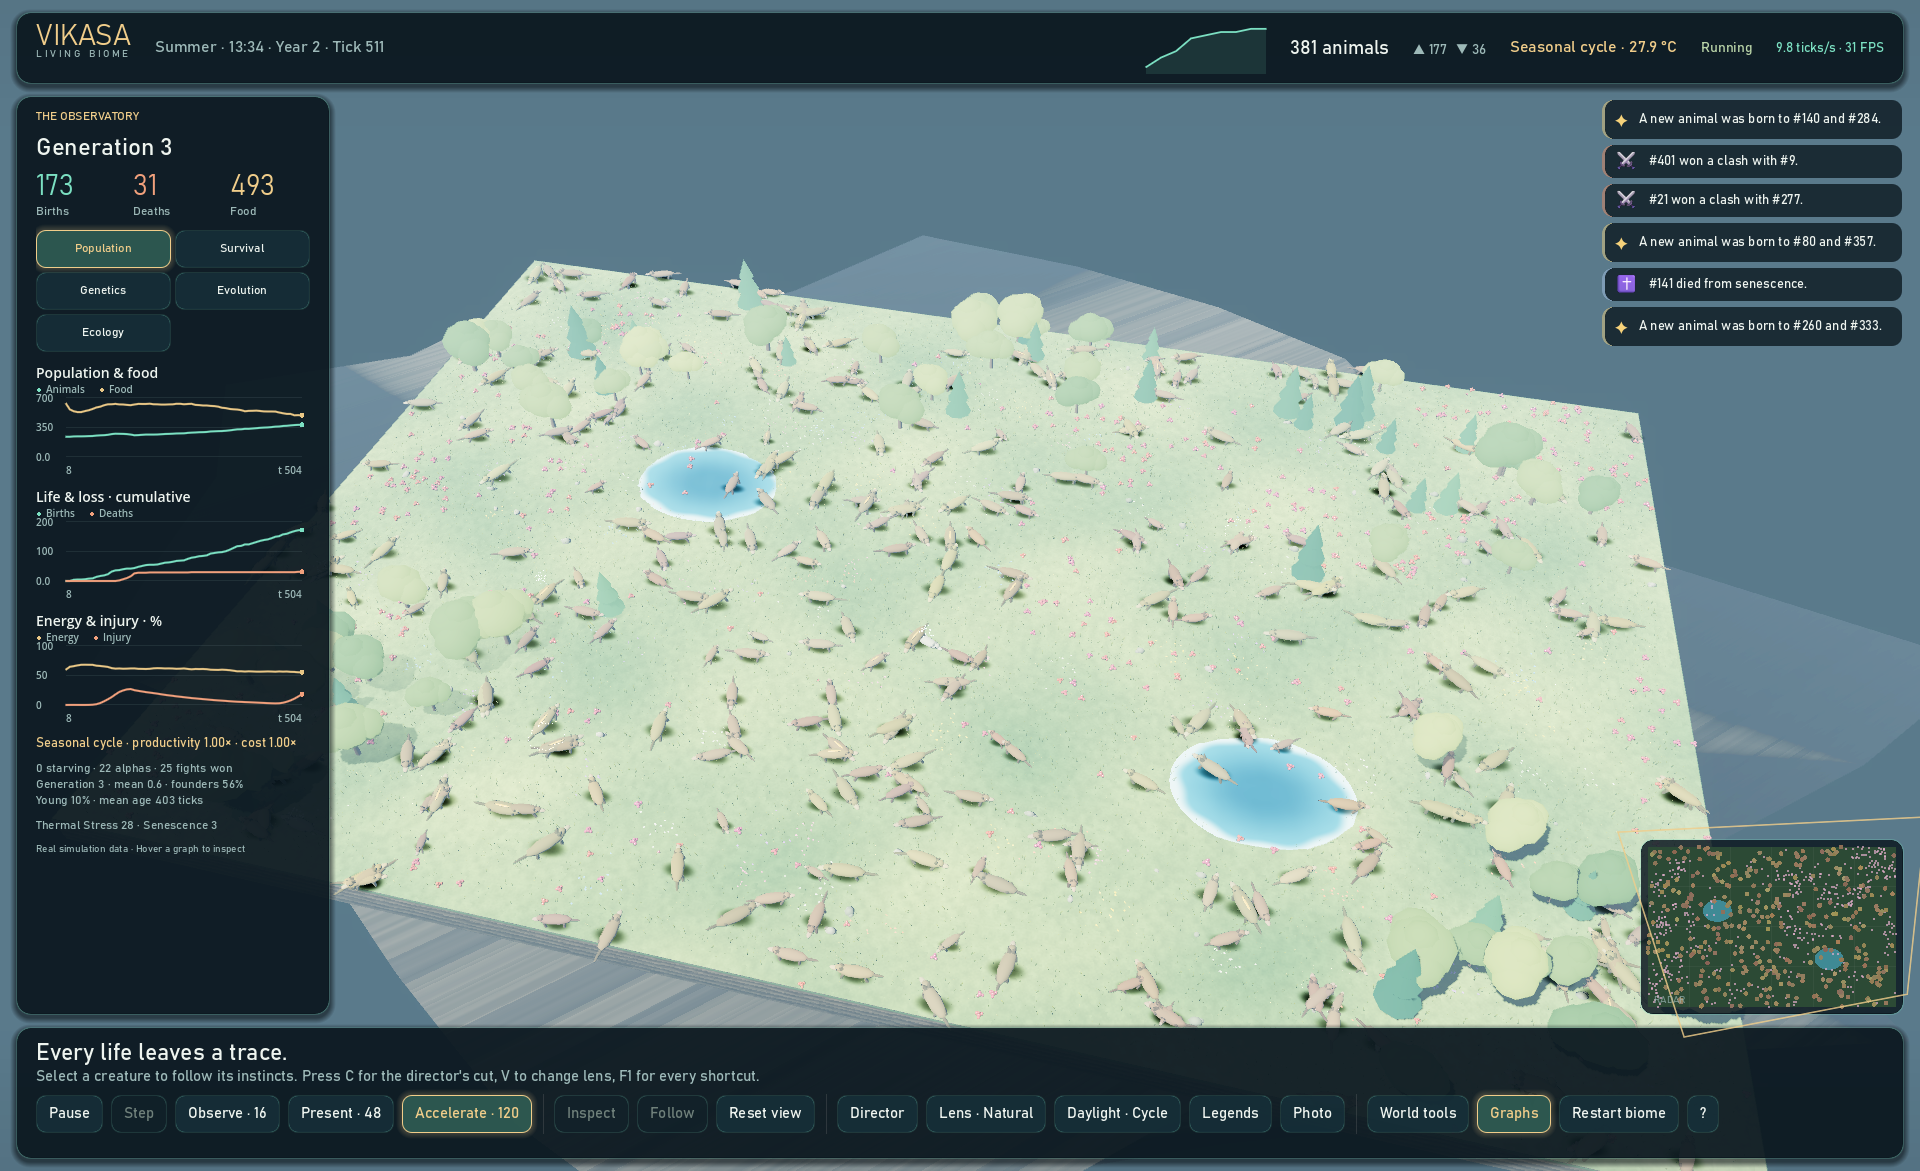
\includegraphics[width=0.55\textwidth]{climate-hud.png}
\caption{Warming demo with live temperature readout.}
\end{figure}

When the estimate and the live check disagree, the live check is the answer. For a
six-year locally adapted species in Hyderabad under SSP5-8.5 the estimate is 58\%
(narrow reference organism) while the live check gives 4 of 4 survivors; the app
shows both and says which to trust.

%===========================================================
\chapter{Conservation Planner}
\label{ch:planner}
%===========================================================

\section{Purpose}
Conservation teams work from a watchlist and a fixed budget. The planner answers
which species to act on first, by when and how, from Vikasa's measured rescue
results. It is a screening tool for prioritising field work, not a substitute for it.

\begin{figure}[htbp]
\centering
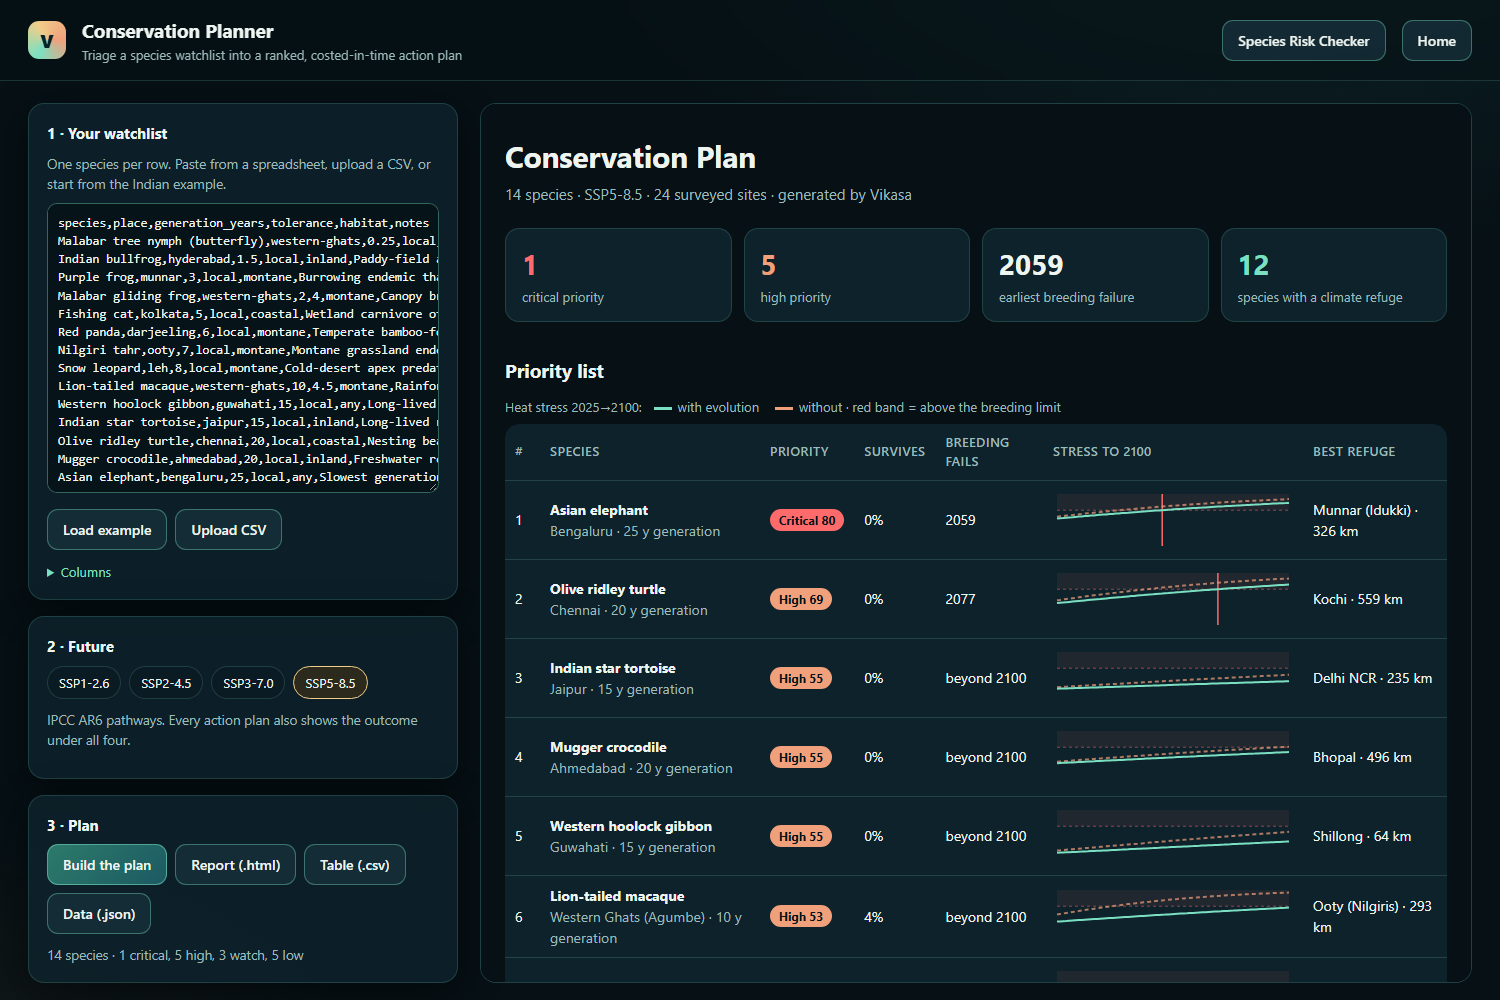
\includegraphics[width=0.85\textwidth]{conservation-planner.png}
\caption{Conservation Planner browser app with the Indian example watchlist.}
\end{figure}

\section{The adaptation-lag model}
For each year $y=2025,\dots,2100$:
\begin{enumerate}[leftmargin=*]
\item Climate is the place's monthly climatology plus the SSP anomaly for $y$.
\item With evolution, the optimum follows warming at the tracking rate
$\min(\dot T_{\text{SSP}},\,k_c/G_{\text{yr}})$, i.e.\ $\theta(y)=\bar T+\text{track}\cdot\max(0,y-2005)$;
without evolution it stays at $\bar T$.
\item Worst-month stress uses the asymmetric rule (warm side $0.6\omega$).
\item Breeding fails in the first year stress exceeds $0.75$ (breeding limit 0.7
plus the 0.05 borderline band), so a borderline place is not reported as failing in 2025.
\end{enumerate}

\section{Interventions}
\textbf{Assisted gene flow.} If no help is needed the shift is 0. Otherwise a grid
in 0.25\,$^{\circ}$C steps up to 15\,$^{\circ}$C finds the first sufficient shift,
then 18 bisection steps refine it, and the answer is rounded \emph{up} to 0.01 so a
reported shift never falls short. \code{None} means no shift works because the
seasonal swing is too wide for the tolerance. Donor sites are places 0--4\,$^{\circ}$C
warmer than home plus the needed shift.

\textbf{Refuges.} Translocated stock keeps its home optimum and is conservatively
not credited with adapting to the new site. A site is a \emph{refuge} if stress
stays under the failure line every year 2030--2100, a \emph{future refuge} if too
cold today but suitable by 2100, and otherwise unsuitable. The optional habitat
(\code{coastal}, \code{montane}, \code{inland}, \code{any}) restricts candidate sites;
distances are great-circle kilometres.

\section{Priority and tiers}
\[
\text{priority}=100\Big(0.55\,(1-p_{\text{surv}})+0.45\cdot\mathrm{clip}\Big(\frac{2100-y_{\text{fail}}}{75}\Big)\Big),
\]
with urgency 0 if breeding never fails. Not viable today gives 100; failure by 2050
gives at least 70. Tiers: Critical $\ge70$, High $\ge45$, Watch $\ge20$, Low below.
The action list is rule-based: gene flow, migration, protecting microrefugia and
corridors, and, when the survival curve and the timeline disagree, ``Confirm with
the live simulation'' first.

\section{Watchlist format and outputs}
CSV columns: \code{species}, \code{place}, \code{generation\_years} (required);
\code{tolerance}, \code{habitat}, \code{ssp}, \code{notes} (optional). Up to 200 rows;
bad rows are reported and skipped. \code{vikasa plan triage} writes a
self-contained \code{report.html} (no scripts, no network, prints cleanly),
\code{plan.csv} and \code{plan.json} (schema \code{vikasa-conservation-plan-v1}).
Twenty-four NASA POWER sites are searched: the seven cities, three study regions
and fourteen survey sites (Ooty, Munnar, Kochi, Pune, Nagpur, Bhopal, Ahmedabad,
Lucknow, Guwahati, Shillong, Darjeeling, Dehradun, Srinagar, Leh).

{\small
\begin{longtable}{clllcl}
\caption{Example triage, \code{examples/watchlist-india.csv}, SSP5-8.5 (illustrative generation times)}\\
\toprule
\# & Species & Place & Tier & Score & First action \\
\midrule
\endfirsthead
\toprule
\# & Species & Place & Tier & Score & First action \\
\midrule
\endhead
1 & Asian elephant & Bengaluru & Critical & 80 & Gene flow +1.3\,$^{\circ}$C \\
2 & Olive ridley turtle & Chennai & High & 69 & Gene flow +0.66\,$^{\circ}$C \\
3 & Indian star tortoise & Jaipur & High & 55 & Confirm with live simulation \\
4 & Mugger crocodile & Ahmedabad & High & 55 & Confirm with live simulation \\
5 & Western hoolock gibbon & Guwahati & High & 55 & Confirm with live simulation \\
6 & Lion-tailed macaque & Western Ghats & High & 53 & Confirm with live simulation \\
7 & Snow leopard & Leh & Watch & 44 & Confirm with live simulation \\
8 & Nilgiri tahr & Ooty & Watch & 35 & Confirm with live simulation \\
9 & Red panda & Darjeeling & Watch & 23 & Protect microrefugia \\
10 & Fishing cat & Kolkata & Low & 13 & Protect microrefugia \\
11 & Purple frog & Munnar & Low & 3 & Routine monitoring \\
12 & Indian bullfrog & Hyderabad & Low & 1 & Run the live check \\
13 & Malabar gliding frog & Western Ghats & Low & 1 & Routine monitoring \\
14 & Malabar tree nymph & Western Ghats & Low & 0 & Routine monitoring \\
\bottomrule
\end{longtable}}

For the elephant, breeding fails in 2059 with evolution and 2046 without, and the
best refuge is Munnar (326\,km); for the olive ridley, 2077 versus 2054, refuge
Kochi (559\,km).

\begin{figure}[htbp]
\centering
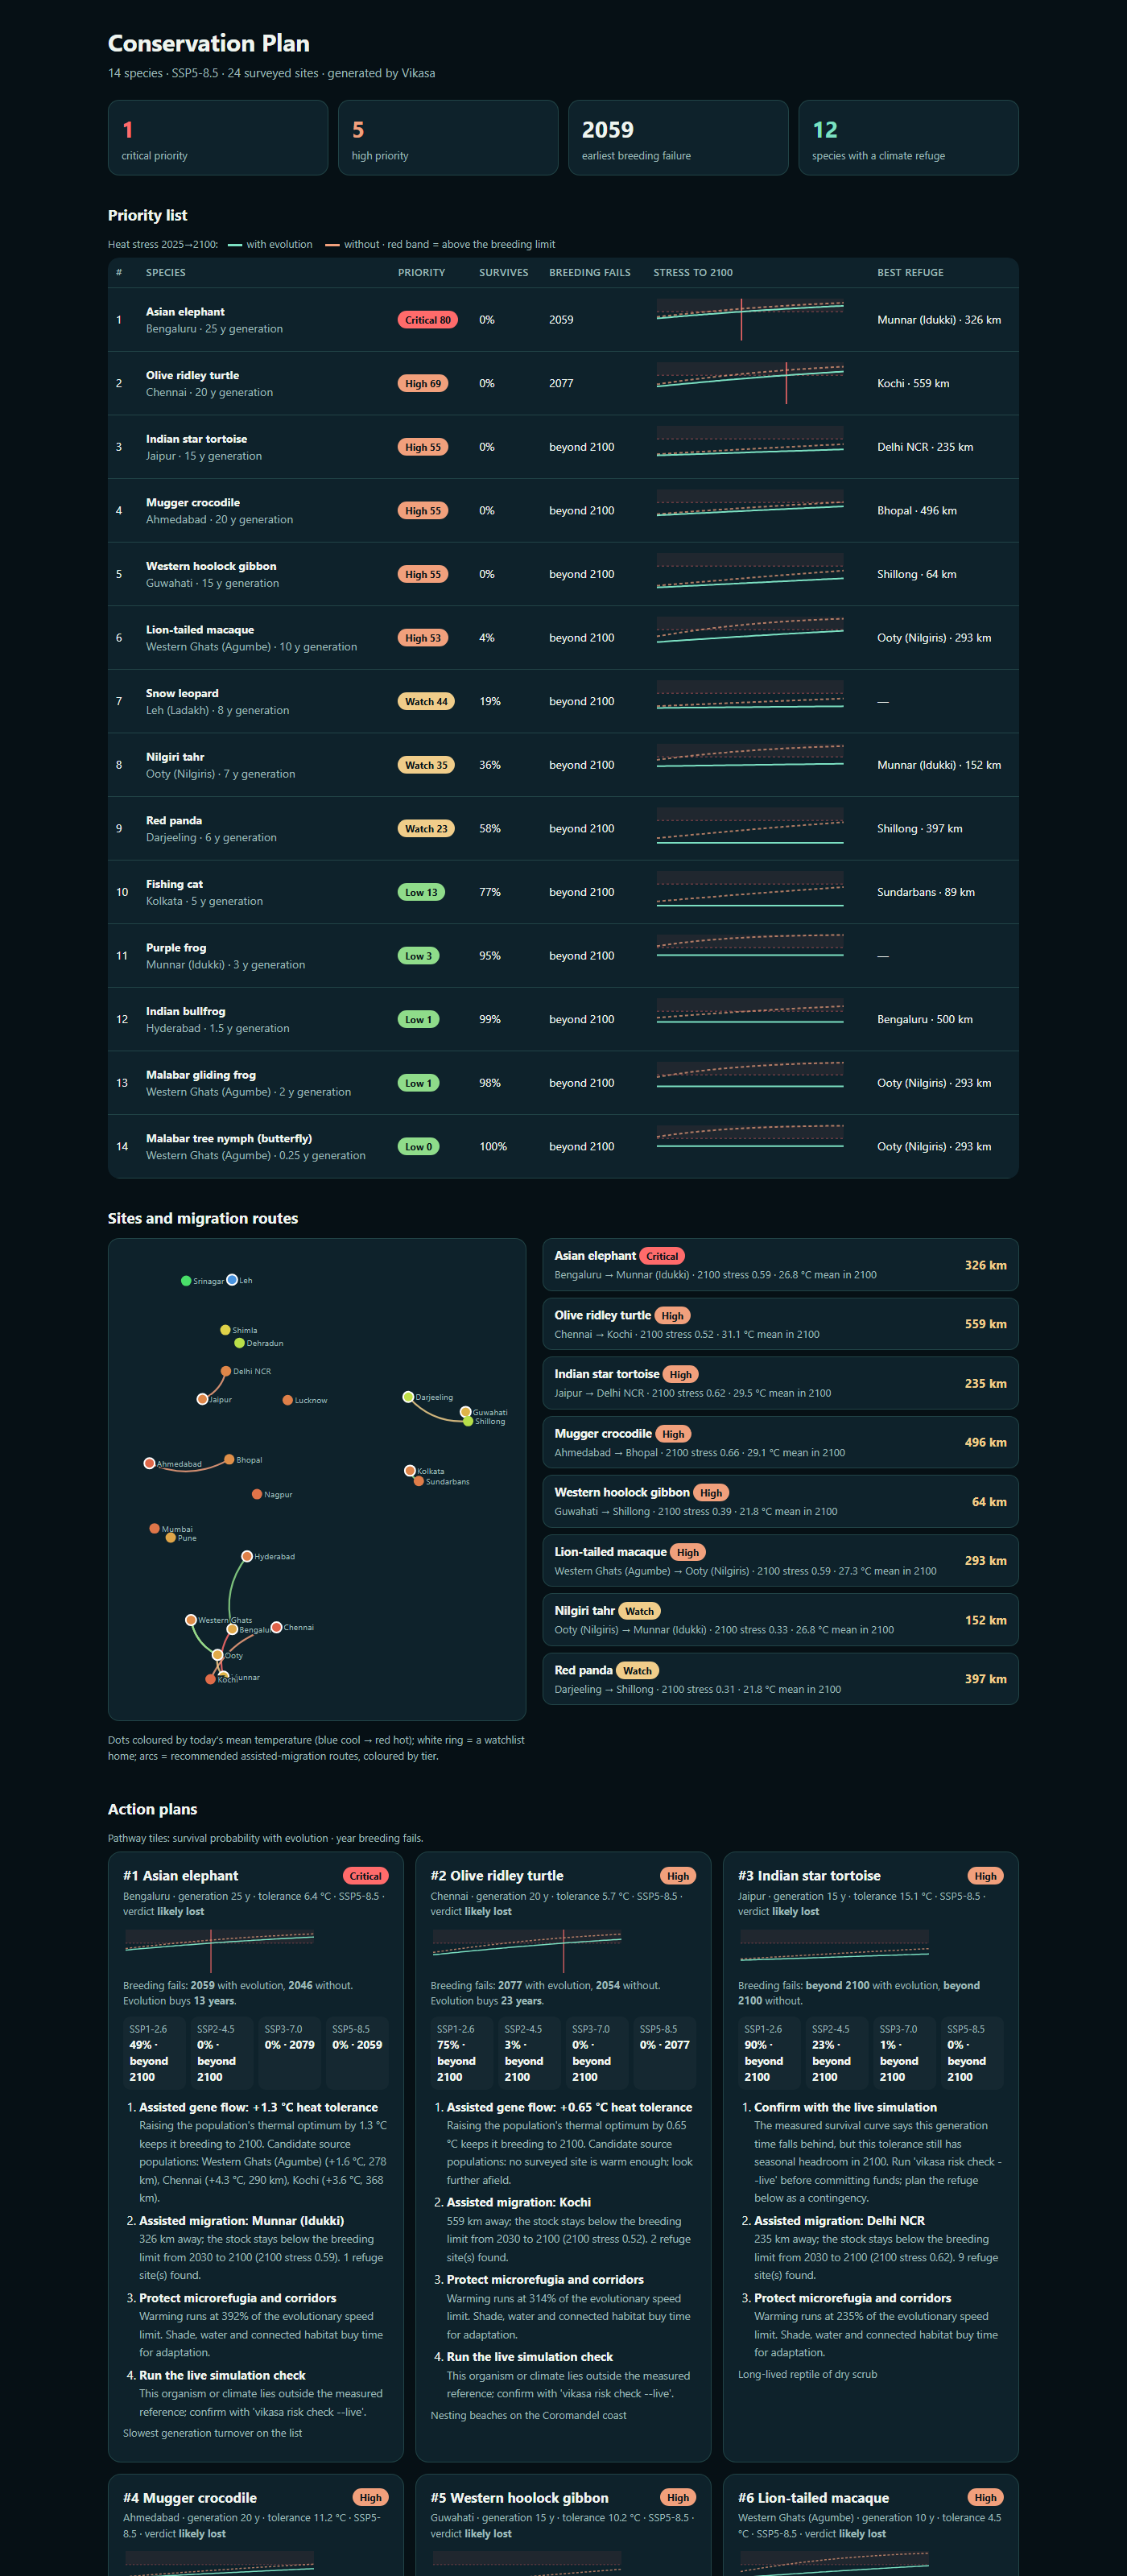
\includegraphics[height=0.42\textheight]{conservation-report.png}
\caption{Self-contained conservation plan report: priority list, migration routes and action cards.}
\end{figure}
